\documentclass{article}
\usepackage{tikz}

\begin{document}

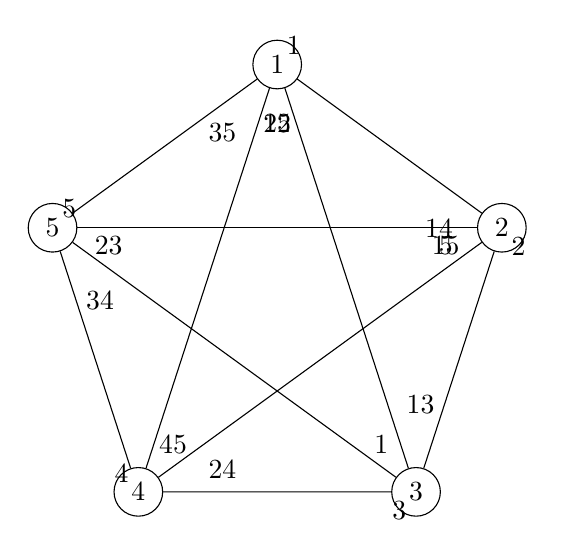
\begin{tikzpicture}[scale=1.5]
    % Define coordinates for the vertices
    \foreach \i in {1,...,5} {
        \pgfmathsetmacro{\angle}{90 - 72 * (\i - 1)}
        \node[circle,draw] (v\i) at (\angle:2cm) {\i};
    }
    
    % Draw edges between vertices
    \draw (v1) -- (v2) -- (v3) -- (v4) -- (v5) -- (v1);
    \draw (v1) -- (v3);
    \draw (v2) -- (v4);
    \draw (v3) -- (v5);
    \draw (v4) -- (v1);
    \draw (v5) -- (v2);
    
    % Add labels to the vertices
    \node at (v1) [above right] {$1$};
    \node at (v2) [below right] {$2$};
    \node at (v3) [below left] {$3$};
    \node at (v4) [above left] {$4$};
    \node at (v5) [above right] {$5$};
    
    % Add labels to the inner nodes
    \node at (90:1.5cm) {$25$};
    \node at (-36:1.5cm) {$13$};
    \node at (-108:1.5cm) {$24$};
    \node at (-180:1.5cm) {$34$};
    \node at (-252:1.5cm) {$35$};
    \node at (-336:1.5cm) {$14$};
    
    % Add labels to the outer nodes
    \node at (18:1.5cm) {$15$};
    \node at (90:1.5cm) {$12$};
    \node at (162:1.5cm) {$23$};
    \node at (234:1.5cm) {$45$};
    \node at (306:1.5cm) {$1$};
    \node at (378:1.5cm) {$5$};
\end{tikzpicture}

\end{document}